\chapter{Test}

\section{Modultest}

\subsection{Software}

\subsubsection{Modultest af Wii-Nunchuck}
På PSoC0 er der software til aflæsning af Wii-Nunchuck input data. Følgende afsnit beskriver test af dette software.

Aflæsning af Wii-Nunchuck sker i to skridt, som begge verificeres ved modul test. Først skal der sendes et \textit{Handshake} fra PSoC0 til Wii-Nunchuck for at initialisere data udveksling, og herefter sker data udveksling hver gang PSoC0 sender en anmodning om det. Disse to skridt modultestes her.

\textbf{Test af Wii-Nunchuck Handshake}

\textbf{Test af data udveksling mellem PSoC0 og Wii-Nunchuck} 

PSoC0 blev programmeret til kontinuert aflæsning af Wii-Nunchuck. For at verificere data udveksling mellem PSoC0 og Wii-Nunchuck blev I2C bussen målt ved brug af Logic Analyzer fra Analog Discovery.

Data udveksling sker i to skridt. Først sender PSoC0 en byte med værdien 0 (0x00 i hexadecimal). Herefter sker den faktiske aflæsning, PSoC0 aflæser Wii-Nunchuck. Begge skridt testes her.

\textbf{Afsendelse af 0x00 byte}

Den første forventede I2C besked er en \textit{0x00} byte fra PSoC0 for at starte en ny aflæsning. På figur \ref{fig:NunchuckWriteValues} ses aflæsningen af I2C bussen på tidspunktet hvor anmodningen til Wii-Nunchuck bliver udført. Dette er en tidslinje læst fra ventre til højre.

\begin{figure}[H]
	\centering
	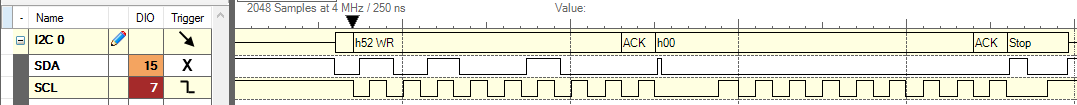
\includegraphics[width=\textwidth]{Test/images/writerequest}
	\caption{}
	\label{fig:NunchuckWriteValues}
\end{figure}

Det kan på figur \ref{fig:NunchuckWriteValues} ses at den første besked der måles er af typen "WR" (Write) til addressen 0x52 (Wii-Nunchuck I2C Slave Addressen). Hertil kommer et tilhørende \textit{ACK} (Acknowledge) fra Wii-Nunchuck. Til sidst sendes dataen Ox00 efterfulgt af at ACK fra Wii-Nunchuck. Til sidst afsluttes I2C transaktionen ved "Stop".

Det kan altså konkluderes at målingen er i overensstemmelse med forventningen om at en 0x00 byte skal sendes til Wii-Nunchuck for opstart af dataudveksling.

\textbf{Aflæsning af Wii-Nunchuck}

Efter vellykket afsendelse af 0x00 byten sker den egentlige aflæsning af Wii-Nunchuk input dataen.

Her forventes en række beskeder indeholdende 

På figur \ref{fig:NunchuckReadValues} ses I2C beskederne der bliver udvekslet mellem PSoC0 og Wii-Nunchuck efter vellykket Wii-Nunchuck Handshake. 

\begin{figure}[H]
	\centering
	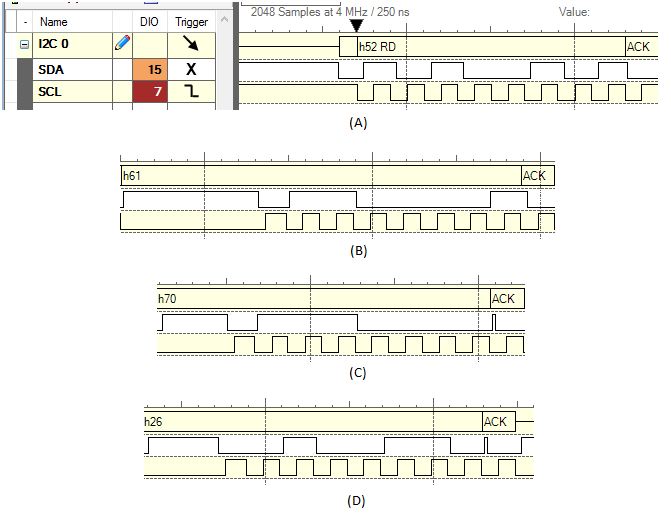
\includegraphics[width=\textwidth]{Test/images/readvaluesEdited.png}
	\caption{Tidslinje af aflæste I2C beskeder af PSoC0 fra Wii-Nunchuck}
	\label{fig:NunchuckReadValues}
\end{figure}

\subsubsection{SPI Protokol}
Devkittet kommunikerer over en SPI bus via SPI protokollen via SPI protokollen i afsnit {\large reference to SPIprotokol}. Dette afsnit beskriver test af denne protokol.

\subsubsection{SPI Bus Test}
Test af SPI bussen udføres i to dele. Første del af testen udføres ved at sende kommandotypen for start af SPI test i terminalen. Derefter måles retur beskeden på bussen med Analog Discovery. Anden del af testen udføres ved at afkoble en fysisk forbindelse på SPI bussen, derefter sendes kommandotypen for start SPI test via terminalen. På terminalen aflæses returbeskeden.

\begin{figure}[H]
	\centering
	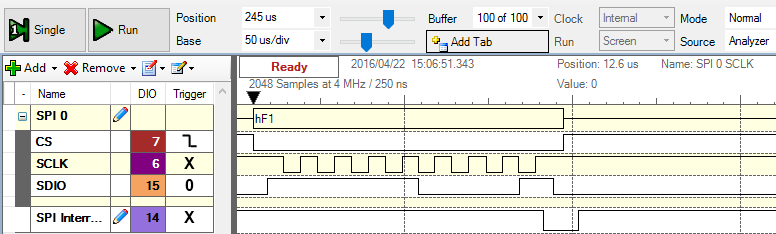
\includegraphics[width=\textwidth]{Test/images/SPItest/SPItestkommandotype}
	\caption{Måling af kommandotype for start SPI test}
	\label{fig:SPItestkommandotype}
\end{figure}

I testen afsendes SPI test kommandotypen, som har værdien 0xF1. Målingen af dette ses i figur \ref{fig:SPItestkommandotype}

\subsubsection{SPI Bus Test: Del 1}
Når kommandotypen er afsendt er det forventede resultat af næste måling på SPI bussen, 0xD1. Måling af returbeskeden ses på figur \ref{fig:SPItestSPIOK}

\begin{figure}[H]
	\centering
	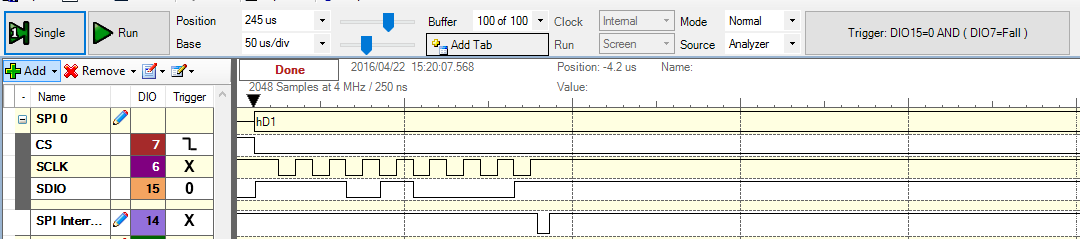
\includegraphics[width=\textwidth]{Test/images/SPItest/SPItestSPIOK1}
	\caption{Måling af returbesked for start SPI test} 
	\label{fig:SPItestSPIOK}
\end{figure}

På figur \ref{fig:SPItestSPIOK} ses at returbeskeden har den forventede værdi 0xD1, som indikerer at SPI bus testens første del er gennemført uden fejl.

\subsubsection{SPI Bus Test: Del 2}
Når kommandotypen er afsendt er det forventede resultat at SPI testen fejler ved at der aflæses en værdi forskellig fra den forventede værdi, 0xD1. På figur \ref{fig:SPItestFAIL}
ses målingen af returbeskeden.

\begin{figure}[H]
	\centering
	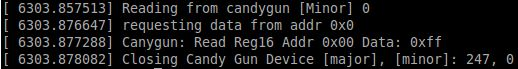
\includegraphics[width=\textwidth]{Test/images/SPItest/SPItestFAIL}
	\caption{Måling af returbesked for start SPI test}
	\label{fig:SPItestFAIL}
\end{figure}

På figur \ref{fig:SPItestFAIL} ses returbeskeden i terminalen ikke har den forventede værdi, 0xD1. Derimod har denne værdien 0xFF, som indikerer at SPI bus testens anden del er gennemført uden fejl.

Ud fra testenes resultater kan det konkluderes at implementeringen af SPI protokollen fungerer efter hensigten.



\subsubsection{I2C Protokol}
PSoC0 og PSoC1 kommunikerer over en I2C bus via I2C protokollen beskrevet i afsnit \ref{afsnit:I2CProtokol}. Dette afsnit beskriver test af denne protokol. Følgende test tager udgangspunkt i kommandotypen \textit{NunchuckData} beskrevet i tabel \ref{table:I2CKommandoer}).

\subsubsection{Test af NunchuckData kommandotype} 

Testen blev udført i to dele. I første del måles I2C bussen ved brug af Analog Discovery's Logic Analyzer; for at verificere at den forventede kommandotype bliver overført via bussen. Anden del verificerer at den overførte data er modtaget korrekt via PSoC Creator's debugger.

\subsubsection{NunchuckData kommandotype test del 1}

I testen afsendes, som nævnt i afsnittets indledning, kommandotypen NunchuckData. Som vist i tabel \ref{table:I2CKommandoer} har denne kommandotype ID'et 0xA2, hvor de efterfølgende 3 data bytes indeholder input dataen fra Wii-Nunchuck.

Det forventede resultat af målingen er at første byte er kommandoentypens ID, som har værdien 0x2A. Kommandoens data - de efterfølgende bytes - verificeres først i anden del, disse indgår altså ikke i følgende måling. 

Målingen ses på figur \ref{fig:NunchuckDataCommand}.

\begin{figure}[H]
	\centering
	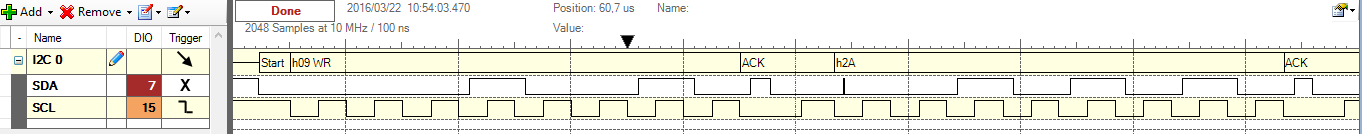
\includegraphics[width=1.2\textwidth]{Test/images/ShowsNunchuckDataCommand.png}
	\caption{Tidslinje af målt I2C kommandotype}
	\label{fig:NunchuckDataCommand}
\end{figure}

Det kan ses på figur \ref{fig:NunchuckDataCommand} at I2C overførslen starter med en I2C \textit{write}, som får et successfuldt acknowledge fra slaven PSoC1. Herefter kan det ses at den næste byte der sendes har værdien 0x2A. Denne byte er kommandoentypens ID, og er altså som forventet 0x2A.

Det kan altså verificeres at kommandoen overføres via I2C bussen. Dataens integritet er dog ikke inkluderet i denne del, og testes i del 2.

\subsubsection{NunchuckData kommandotype test del 2}
For at verificere integriteten af den data der sendes mellem PSoC0 og PSoC1, bruges PSoC Creators indbyggede debugger. Igen er det kommandotypen NunchuckData der sendes mellem de to enheder, hvor de medfølgende data bytes fortolkes.

Testen gennemføres ved at fortolke den modtagne data tre gange, hvor nunchucken er i forskellige tilstande (hvilken retning det analoge stik er trykket) i hver test. Værdierne sammenlignes de forventede standardværdier som ses i tabellen på side 3 i \cite[I2C Interface with Wii Nunchuck]{nunchuck}. Da testene kun er fokuserede på, hvilken retning den analoge stick er presset, er det altså kun receivedDataBuffer[1] (den analoge stick x-akse) og receivedDataBuffer[2] (den analoge pinds y-akse) der er relevante for testen. Når den analoge stick er presset til venstre, forventes det ifølge tabel \ref{tabel:WiiNunchuckStickPositioner} at receivedDataBuffer[1] er lig 0x1E og receivedDataBuffer[2] er 0x7B. Når den analoge stick er presset op, forventes det at receivedDataBuffer[1] er 0x7E og receivedDataBuffer[2] er 0xDF. Når der ikke er noget input på Nunchucken forventes det at receivedDataBuffer[1] er 0x7E og receivedDataBuffer[2] er 0x7B. Målingerne for testene kan ses på figur \ref{fig:I2CProtocolReadNoInput}, \ref{fig:I2CProtocolReadLeftAnalog} og \ref{fig:I2CProtocolReadUpAnalog}.

\begin{figure}[H]
	\centering
	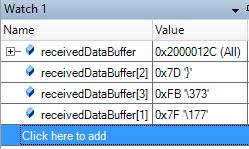
\includegraphics[width=.5\textwidth]{Test/images/I2CProtocolReadNoInput.png}
	\caption{Afmåling af modtager-buffer på PSoC1 efter at have modtaget "NunchuckData" kommando typen. Intet input på Nunchuck'en}
	\label{fig:I2CProtocolReadNoInput}
\end{figure}

\begin{figure}[H]
	\centering
	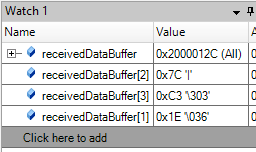
\includegraphics[width=.5\textwidth]{Test/images/I2CProtocolReadLeftAnalog.png}
	\caption{Afmåling af modtager-buffer på PSoC1 efter at have modtaget "NunchuckData" kommando typen. Den analoge stick er presset til venstre på Nunchuck'en}
	\label{fig:I2CProtocolReadLeftAnalog}
\end{figure}

\begin{figure}[H]
	\centering
	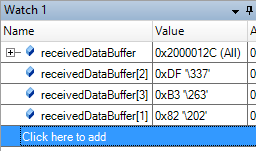
\includegraphics[width=.5\textwidth]{Test/images/I2CProtocolReadUpAnalog.png}
	\caption{Afmåling af modtager-buffer på PSoC1 efter at have modtaget "NunchuckData" kommando typen. Den analoge stick er presset frem på Nunchuck'en}
	\label{fig:I2CProtocolReadUpAnalog}
\end{figure}

På figur \ref{fig:I2CProtocolReadLeftAnalog} ses afmålingen af modtager-bufferen når Nunchuckens analoge stick er presset helt til venstre. ReceivedDataBuffer[1] blev aflæst til 0x1E og receivedDataBuffer[2] blev aflæst til 0x7C. ReceivedDataBuffer[1] stemmer overens med forventningerne. ReceivedDataBuffer[2] har en lille afvigelse (oversat til decimaltal blev der målt 124, hvor der forventes 123). Denne afvigelse kan skyldes, at det analoge stick ikke blev presset direkte til venstre, men at den også er blevet presset en smule frem under målingen.

På figur \ref{fig:I2CProtocolReadUpAnalog} ses afmålingen af modtager-bufferen når Nunchuckens analoge stick er presset frem. ReceivedDataBuffer[1] blev aflæst til 0x82, hvor det var forventet 0x7E. Dette er en afvigelse fra de forventede resultater med 4, og kan skyldes at det analoge stick ikke var helt centreret idét den blev presset frem under målingen. ReceivedDataBuffer[2] blev aflæst til 0xDF, hvilket stemmer overens med de forventede målinger.

På figur \ref{fig:I2CProtocolReadNoInput} ses afmålingen af modtager-bufferen når der ikke er noget brugerinput på nunchuckens analoge stick. ReceivedDataBuffer[1] blev aflæst til 0x7F, hvor det forventede resultat var 0x7E. Denne afvigelse kan skyldes at det analoge stick ikke stod helt i midten under målingen (Det analoge stick er lidt "løs" og kan defor godt finde hvile i en position der ikke er fuldt centreret). ReceivedDataBuffer[2] blev aflæst til 0x7D, hvor det forventede resultat var 0x7B. Igen kan denne afvigelse skyldes at det analoge stick ikke var i centrum under målingen.

Ud fra testen kan det konkluderes at implementeringen af I2C-protokollen fungerer efter hensigten.

\subsection{Hardware}
\subsubsection{H-bro} 

\textbf{Formål}
\\ Formålet med denne test er at viser at motor kan styres i begge retninger, ved hjælp af h broen.\\

\textbf{Overordnet opstilling}

\begin{figure}[H]
	\centering
	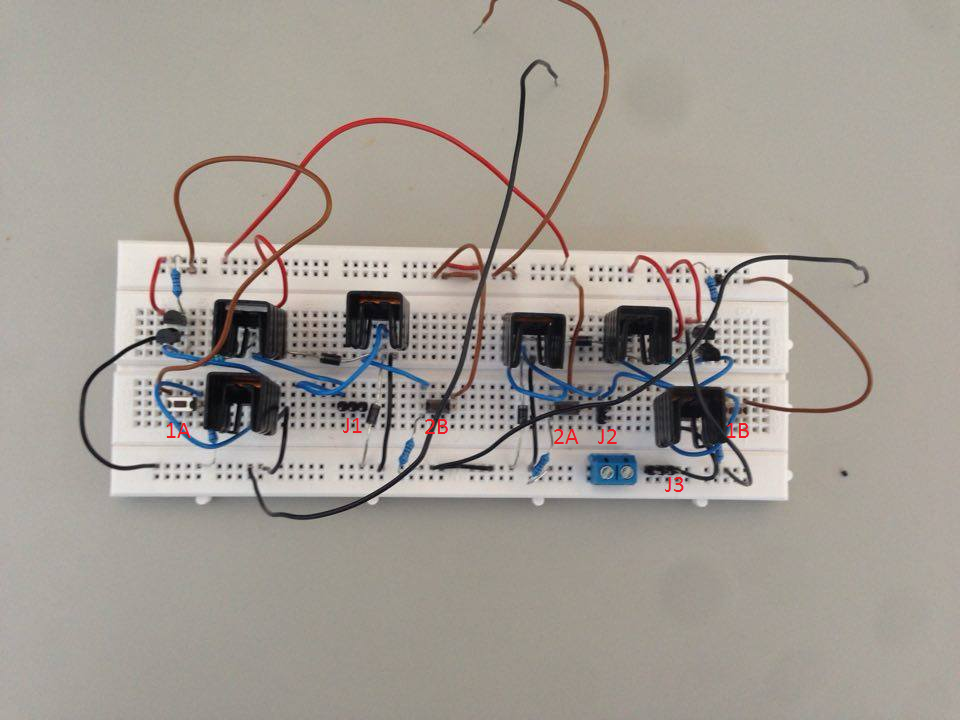
\includegraphics[width=\textwidth]{test/images/testhbroopst}
	\caption{Opstilling af h bro på fumlebræt}
\end{figure}

\begin{itemize}
	\item Røde ledninger er 9 V
	\item	Brune ledninger 5 V
	\item	Blå ledninger er spændinger inde imellem komponenter
	\item	Sort er ground
	\item	J1 og J2 er test pin 
	\item	1a og 2a knapper til at styre motor til højre
	\item	1b og 2b knapper til at styre motor til venstre 
	\item	J3 er ground
	
	\end{itemize}

For at teste om h broen kan styre motoren i begge retninger, blev der sat Analog Discovery på de to test pin (J1, J2 og J3) og der blev sat 5V, 9V og ground til. 
Først del af testen var at tjekke om den kunne køre til højre, det blev gjord ved at trykke på knap 1a og 2a.
Anden del af testen var at tjekke om den kunne køre til venstre det blev gjord ved at trykke på knap 1b og 2b.
\\
\\
\textbf{Forventet resultat}
At når der blev trykket på knap 1a og 2a vil den ene kurv gå høj og den anden vil for blive lav
At når der blev trykket på knap 1b og 2b vil den anden kurv gå høj og den først vil for blive lav.
\\
\\

\textbf{Opnået resultat}
\begin{figure}[H]
	\centering
	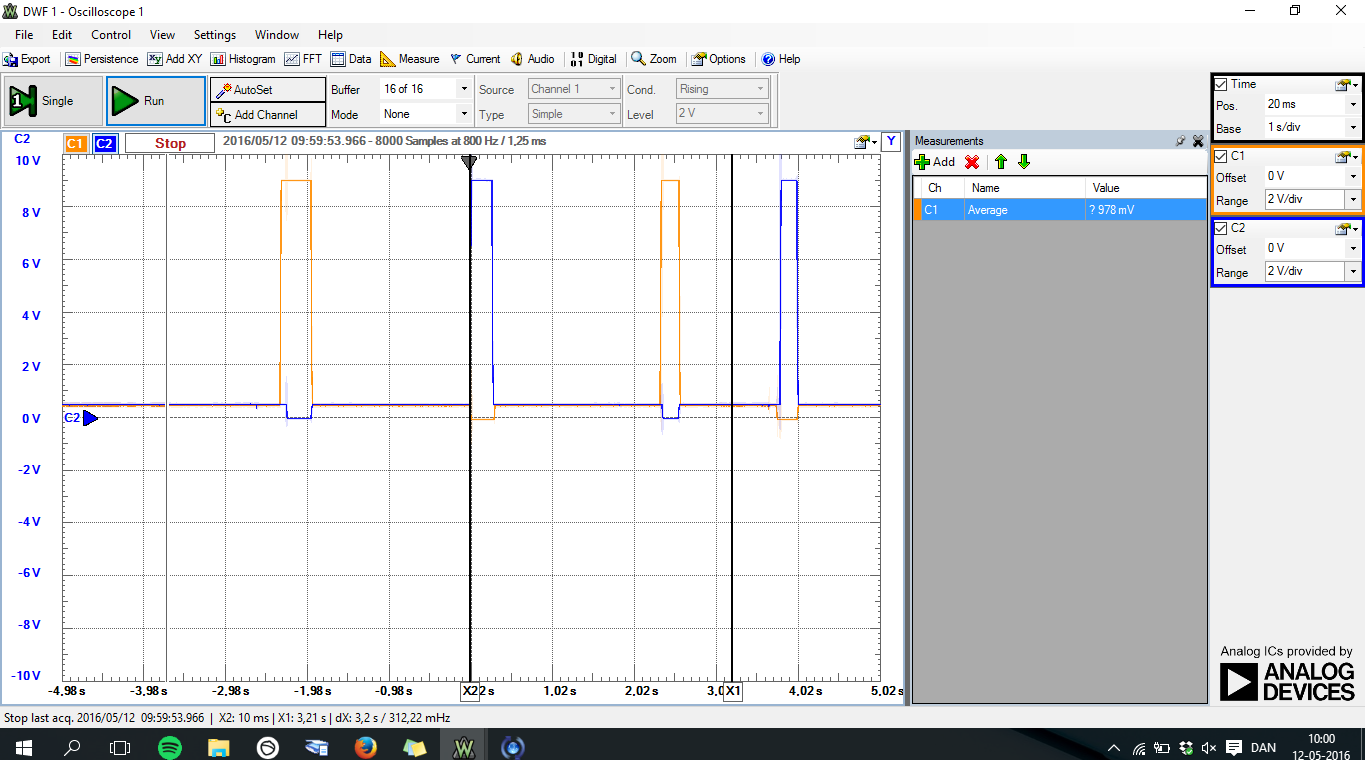
\includegraphics[width=\textwidth]{test/images/testhbro}
	\caption{Modultest for H-bro}
	
\end{figure}
 Som det fremgår på figuren, kan man se at, i det der bliver åbnet for at motor kan køre i den ene retning, så stiger den blå op til 9V fordi nu har den fået forbindelse til ground og fået forbindelse til de 9V. Hvor samtidigt at blå går højt, så går den orange lavere, for nu trækker den blå alt spændingen. Det samme sker når man åbner op for at den kan løbe spændingen kan løbe den anden vej, i stedet for at det er den blå som går høj, er det den orange som går høj. Med det kan man se at motor kan køre i begge retninger uden problemer.
 Der er blevet valgt at der ikke tages billede af at motoren køre, for man ikke se på et billede hvilken vej den køre og overhovedet den køre. Der ses også på figuren at der noget støj, når orange/blå går højt, men det er ikke noget som kommer til at påvirker vores styring af motoren

Man kan også på figuren se at når den orange/blå går høj, så stiger den meget hurtig, grunden til den gør det var på grund af at, der er blevet sat de to transistor ind, får p mosfet, som gør at den bliver opladt hurtigere, end den ellers ville på grund af der sidder en form for kondensatorer inde i den mosfet, som skal have hjælp med at bliv opladt. Det hjælp kommer fra de transistor som er blevet sat ind før Mosfeten.  




\section{Integration}

\section{Accepttest}